%%%%%%%%%%%%%%%%%%%%%%%%%%%%%%%%%%%%%%%%%
% Beamer Presentation
% LaTeX Template
% Version 1.0 (10/11/12)
%
% This template has been downloaded from:
% http://www.LaTeXTemplates.com
%
% License:
% CC BY-NC-SA 3.0 (http://creativecommons.org/licenses/by-nc-sa/3.0/)
%
%%%%%%%%%%%%%%%%%%%%%%%%%%%%%%%%%%%%%%%%%

%----------------------------------------------------------------------------------------
%	PACKAGES AND THEMES
%----------------------------------------------------------------------------------------

\documentclass[c]{beamer}
%\documentclass[notes]{beamer}
\setbeamertemplate{note page}[show only notes]
\input{../OR_common.tex}
%%%%%%%%%%%%%%%%%%%%%%%%%%%%%%%%%%%%%%%%%%%%%%%%%%%%%%%%%%%%%%%%%%%%%%%%%%%%%
%%%%%%%%%%%%%%%%%%%%%%%%%%%%%%%%%%%%%%%%%%%%%%%%%%%%%%%%%%%%%%%%%%%%%%%%%%%%%
%%%%%%%%%%%%%%%%%%%%%%%%%%%%%%%%%%%%%%%%%%%%%%%%%%%%%%%%%%%%%%%%%%%%%%%%%%%%%

\title[Introduction]{Unit 1. Introduction to Operational Research}

\author{Jordi Villà i Freixa}
\institute[FCTE]{
Universitat de Vic - Universitat Central de Catalunya \\
Study Abroad. Operations Research\\
\medskip
\textit{jordi.villa@uvic.cat}
}
\date{8/02, 2024}
\logo{
\includegraphics[width=.1\textwidth]{FCTE}}
\begin{document}

\begin{frame}
\titlepage
\end{frame}


\begin{frame}
    \frametitle{Preliminary}
    This course is strongly based on the monography on Operations Research by Carter, Price and Rabadi \cite{carter}, and in material obtained from different sources (quoted when needed through the slides).
\end{frame}

%%%%%%%%%%%%%%%%%%%%%%%%%%%%%%%%%%%%%%%%%%%%%%%%%%%%%%%%%%%%%%%%%%%%%%%%%%%%%
%%%%%%%%%%%%%%%%%%%%%%%%%%%%%%%%%%%%%%%%%%%%%%%%%%%%%%%%%%%%%%%%%%%%%%%%%%%%%
%%%%%%%%%%%%%%%%%%%%%%%%%%%%%%%%%%%%%%%%%%%%%%%%%%%%%%%%%%%%%%%%%%%%%%%%%%%%%

\begin{frame}
\frametitle{Learning outcomes}
\begin{itemize}
  \item Learn about the origins and applications of Operations Research
  \item Understand system modelling principles
  \item Understand algorithm efficiency and problem complexity
  \item Contrast between the optimality and practicality
  \item Learn about software for operations Research
  \item Introduction to the Python/Colab environment
\end{itemize}
\end{frame}

%%%%%%%%%%%%%%%%%%%%%%%%%%%%%%%%%%%%%%%%%%%%%%%%%%%%%%%%%%%%%%%%%%%%%%%%%%%%%
%%%%%%%%%%%%%%%%%%%%%%%%%%%%%%%%%%%%%%%%%%%%%%%%%%%%%%%%%%%%%%%%%%%%%%%%%%%%%
%%%%%%%%%%%%%%%%%%%%%%%%%%%%%%%%%%%%%%%%%%%%%%%%%%%%%%%%%%%%%%%%%%%%%%%%%%%%%

\section{Operation research}

\begin{frame}
\begin{block}{Operations research (OR)...}
The use of quantitative methods to assist analysis and decision-makers in designing, analysizing and improving the performance or operation of systems.
\end{block}
\begin{block}{...or}
Applied math field, where mathematical tools and operators aren’t used to investigate mathematics further but rather to analyse and solve problems within the OR domain by designing innovative solution approaches.
\end{block}
Link to a \href{https://towardsdatascience.com/the-big-picture-of-operations-research-8652d5153aad}{big picture view of OR}
\end{frame}

%------------------------------------------------

\begin{frame}
  \begin{center}
    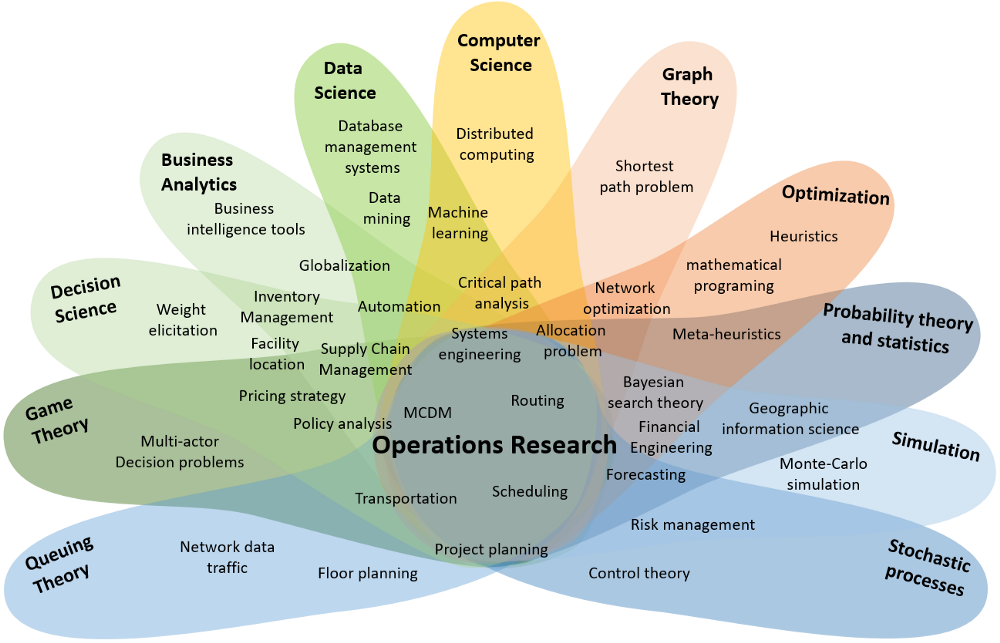
\includegraphics[width=\textwidth]{OR_AlexElkjaer.png}
  \end{center}
\end{frame}

\begin{frame}
  \begin{itemize}
    \item OR incorporates analytical tools from many different disciplines, so that they can be applied in a rational way to help decision-makers solve problems and control operations in practice
    \item OR has been taking shape since the industrial revolution, and most notably after WWII
  \end{itemize}
  The term Operations Research was first coined in 1940 by McClosky and Trefthen
in a small town, Bowdsey, of the United Kingdom, in a military context (the Battle of England).
\end{frame}

\begin{frame}
  \frametitle{System modelling principles}
  \begin{itemize}
    \item A model is a simplified, idealized representation of a real object, a real process, or a real system
    \item In mathematical models, the building blocks are mathematical structures (equations, inequalities, matrices, functions and operators)
    \item Building a model:
          \tikzstyle{decision} = [diamond, draw, fill=blue!20,text width=4.5em, text badly centered, node distance=3cm, inner sep=0pt]
\tikzstyle{block} = [rectangle, draw, fill=blue!20,text width=15em, text centered, rounded corners, minimum height=3em]
\tikzstyle{line} = [draw, -latex']
\tikzstyle{cloud} = [draw, ellipse,fill=red!20, node distance=3cm,minimum height=2em]


\begin{adjustbox}{max totalsize={.9\textheight},center}

  \begin{tikzpicture}[node distance = 2cm, auto,rotate=90,transform shape]
    % Place nodes
    \node [block] (step1) {Area in need of model?};
    \node [block, below of=step1] (step2) {Controllable aspects?};
    \node [block, below of=step2] (step3) {Goals and purpose?};
    \node [block, below of=step3] (step4) {Constraints and limitations?};
    \node [block, below of=step4] (step5) {Create model};
    \node [block, below of=step5] (step6) {Collect data};
    \node [block, below of=step6] (step7) {Solve model and analyse};
    \node [coordinate, above right =1cm and 1cm of step7] (inici){};
    \node [coordinate, below right =1cm and 1cm of step4] (final){};
    % Draw edges
    \path [line] (step1) -- (step2);
    \path [line] (step2) -- (step3);
    \path [line] (step3) -- (step4);
    \path [line] (step4) -- (step5);
    \path [line] (step6) -- (step7);
    \path [line] (step7.east) -| (inici) -- (final) |- (step4.east);
  \end{tikzpicture}

\end{adjustbox}

  \end{itemize}
\end{frame}

\begin{frame}
  \frametitle{The art and science of modeling}
  \begin{itemize}
    \item The best model of a system strikes a practical compromise between being realistic vs understandable and computationally tractable
    \item Detail $\neq$ Accuracy (not all details are correct nor necessary)
    \item A too detailed model brings complexity to analyze it and exploit it
    \item Models need to be realistic and simple
  \end{itemize}
  \epigraph{``Everything should be made as simple as possible, but not simpler"}{Albert Einstein}
\end{frame}


\begin{frame}
  \frametitle{Practical issues in modelling}
  \begin{itemize}
    \item Does the problem need to be solved?
    \item What is the {\it real} problem?
    \item Would the eventual solution to the problem useful for somebody?
    \item Would anybody try to implement the solution?
    \item How much of the analyst's time and cost is worth?
    \item Are there time and resources available to solve the problem?
    \item Will the solution create other serious problems for which there is no apparent remedy?
  \end{itemize}
\end{frame}

\begin{frame}{Problem formulation in Operational Research}
  \begin{columns}
    \begin{column}{0.5\textwidth}

      \begin{description}
        \item[Decision variables] In what are we going to base our decision?
        \item[Objective function] How is our function build with respect to the variables?
        \item[Constraints] What are the limits in our model variables and function?
      \end{description}
    \end{column}
    \begin{column}{0.5\textwidth}
      \begin{center}
        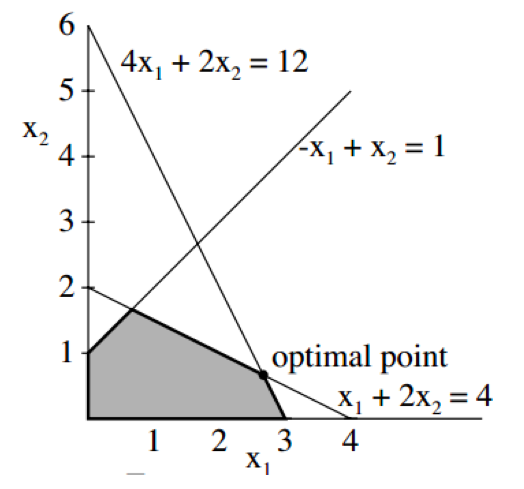
\includegraphics[width=0.8\textwidth]{LP.png}
      \end{center}
    \end{column}
  \end{columns}
\end{frame}

\begin{frame}
  \frametitle{Algorithm efficiency and problem complexity}
  \begin{block}{Algorithm}
    Sequence of operations that can be carried out in a finite amount of time
  \end{block}
  \begin{itemize}
    \item It can be repeated or called recursively but it will eventually terminate.
    \item Factors influencing the execution time (unrelated to the algorthm itself):
    \begin{itemize}
      \item the programming language,
      \item the programmer's skills,
      \item the hardware being used,
      \item the task load on the computer system during execution.
    \end{itemize}
    \item The performance of an algorithm is typically linked to the size of the problem.
  \end{itemize}
\end{frame}

\begin{frame}
  \frametitle{Two types of problems}
  \begin{columns}
    \begin{column}{0.5\textwidth}
  %veure explicació a http://www.solipsys.co.uk/new/PVsNP.html
      \begin{block}{Class P}
        Problems that can be solved by an algorithm within an amount of computation time proportional to some polynomial function of the problem size.
      \end{block}
      \begin{block}{Class NP}
        Problems that require computation time proportional to some exponential (or larger) function of the problem size. (The subset sum problem, for example, is $O(2^n\cdot n$))
        %https://towardsdatascience.com/how-to-find-all-solutions-to-the-subset-sum-problem-597f77677e45, incloent python program
      \end{block}
    \end{column}
    \begin{column}{0.5\textwidth}
      \begin{center}
        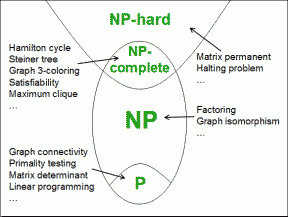
\includegraphics[scale=0.5]{nphard288.png}\\
        \footnotesize{\url{http://www.solipsys.co.uk/new/PVsNP.html}}
      \end{center}
    \end{column}
  \end{columns}
\end{frame}

\begin{frame}
  \frametitle{3-color problem is NP hard}
  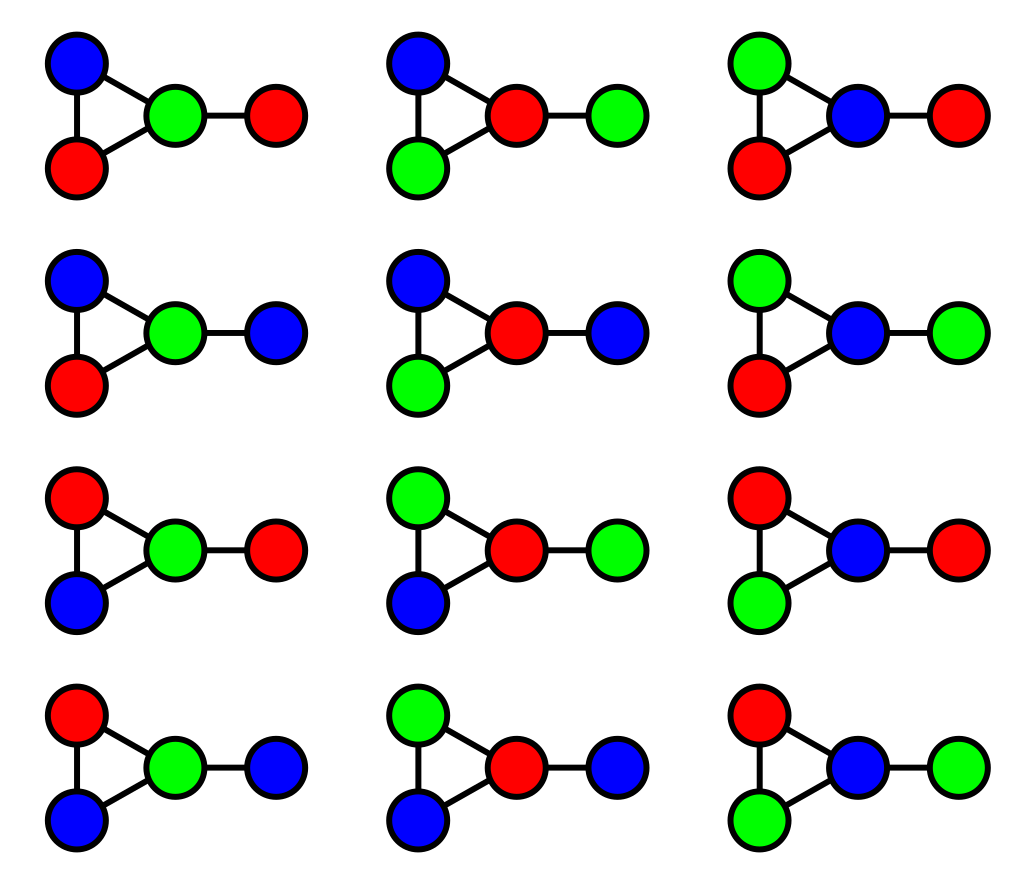
\includegraphics[width=\linewidth]{3colorproblem.png}
\end{frame}

\begin{frame}
  \frametitle{Algorithm efficiency}
  \begin{columns}
    \begin{column}{0.4\textwidth}
      \begin{itemize}
        \item Performance of algorithm independent of software/hardware/developer skill....? \# of computational steps.
        \item Consider worst case scenario: the largest number of steps that may be necessary.
      \end{itemize}
    \end{column}
    \begin{column}{0.6\textwidth}
      \begin{center}
        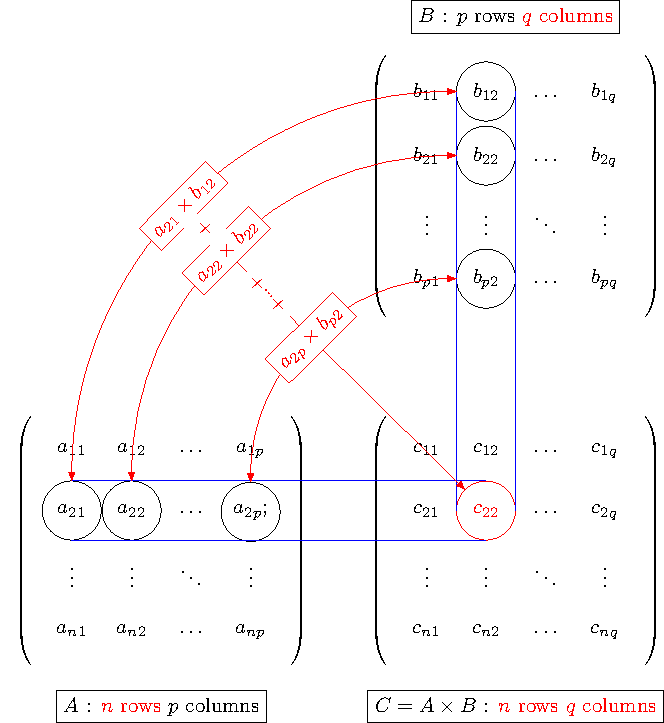
\includegraphics[width=0.7\linewidth]{matrixmultipl.pdf}
      \end{center}
      \footnotesize
      Multiplying two $n\times n$ matrices, in worst case, involves time proportional to $2n^3$.
      \normalsize
    \end{column}
  \end{columns}
\end{frame}



\begin{frame}{Matrix multiplication is $O(n^3)$}
  \begin{footnotesize}
  \lstinputlisting[language=Python]{../code/matrixmultN3.py}
\end{footnotesize}
\end{frame}
%--- Next Frame ---%

\begin{frame}{$O(n)$ notation}
  \begin{itemize}
    \item We say $f(n)=O(g(n))$, and we read as "$f(n)$ is big-O of $g(n)$", if there is some $C$ and $N$ such that
    \[
      |f(n)| \leq C g(n), \; \forall n\geq N.
    \]
    In the previous example, multiplying two $n \times n$ matrices costs $2n^3=O(n^3)$ flops\footnote{FLOating Point operationS per second}. We say the algorithm is of order 3.
    \item $n$ denotes the problem size and $g(n)$ is some function of problem size.
    \item $g(n)$ is the algorithm's worst case step count, as a function of $n$.
    \item $c$ is the constant of proportionality, and accounbts for extraneous factors affecting execution time (hardware speed, programming style, computer system load during execution)
  \end{itemize}
\end{frame}


\begin{frame}{Different orders, different complexity}
  \begin{center}
    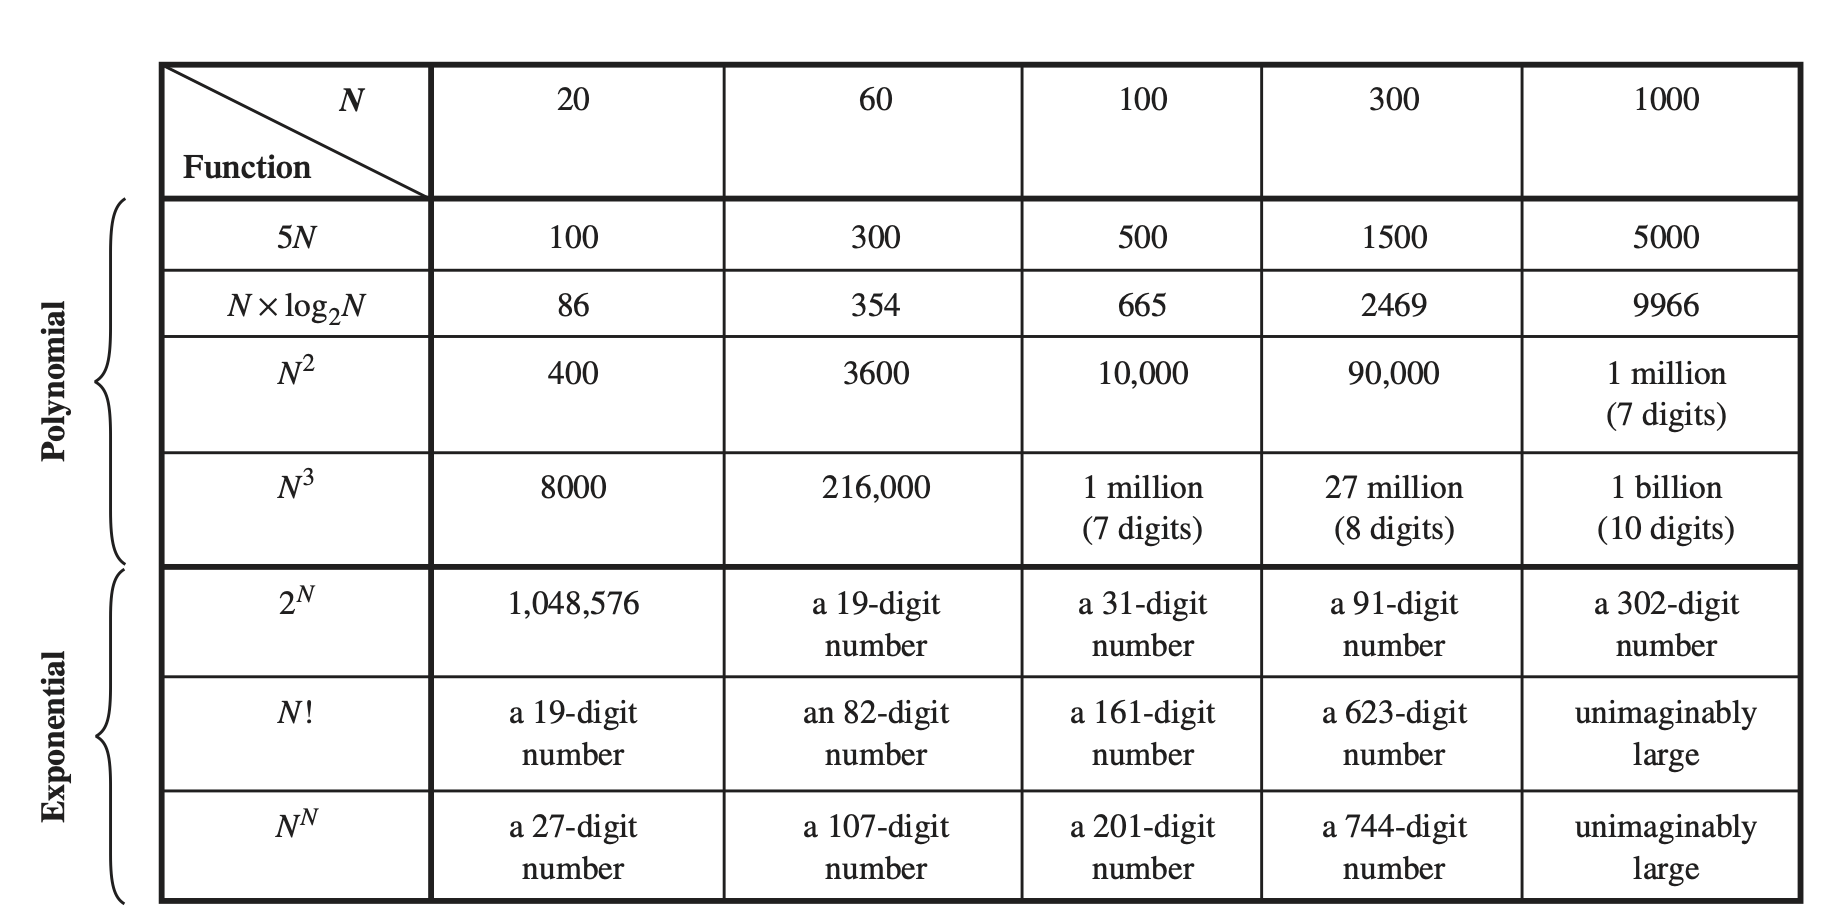
\includegraphics[width=0.8\textwidth]{Harel1.png}
  \end{center}
  Extracted from \cite{harel}
\end{frame}

\begin{frame}[t]{Growth rate of some functions}
  \begin{columns}
    \begin{column}{0.4\textwidth}
      For comparison: the number of protons in the known universe has 79 digits; the number of nanoseconds since the Big Bang has 27 digits.\cite{harel}
    \end{column}
    \begin{column}{0.5\textwidth}
      \begin{center}
        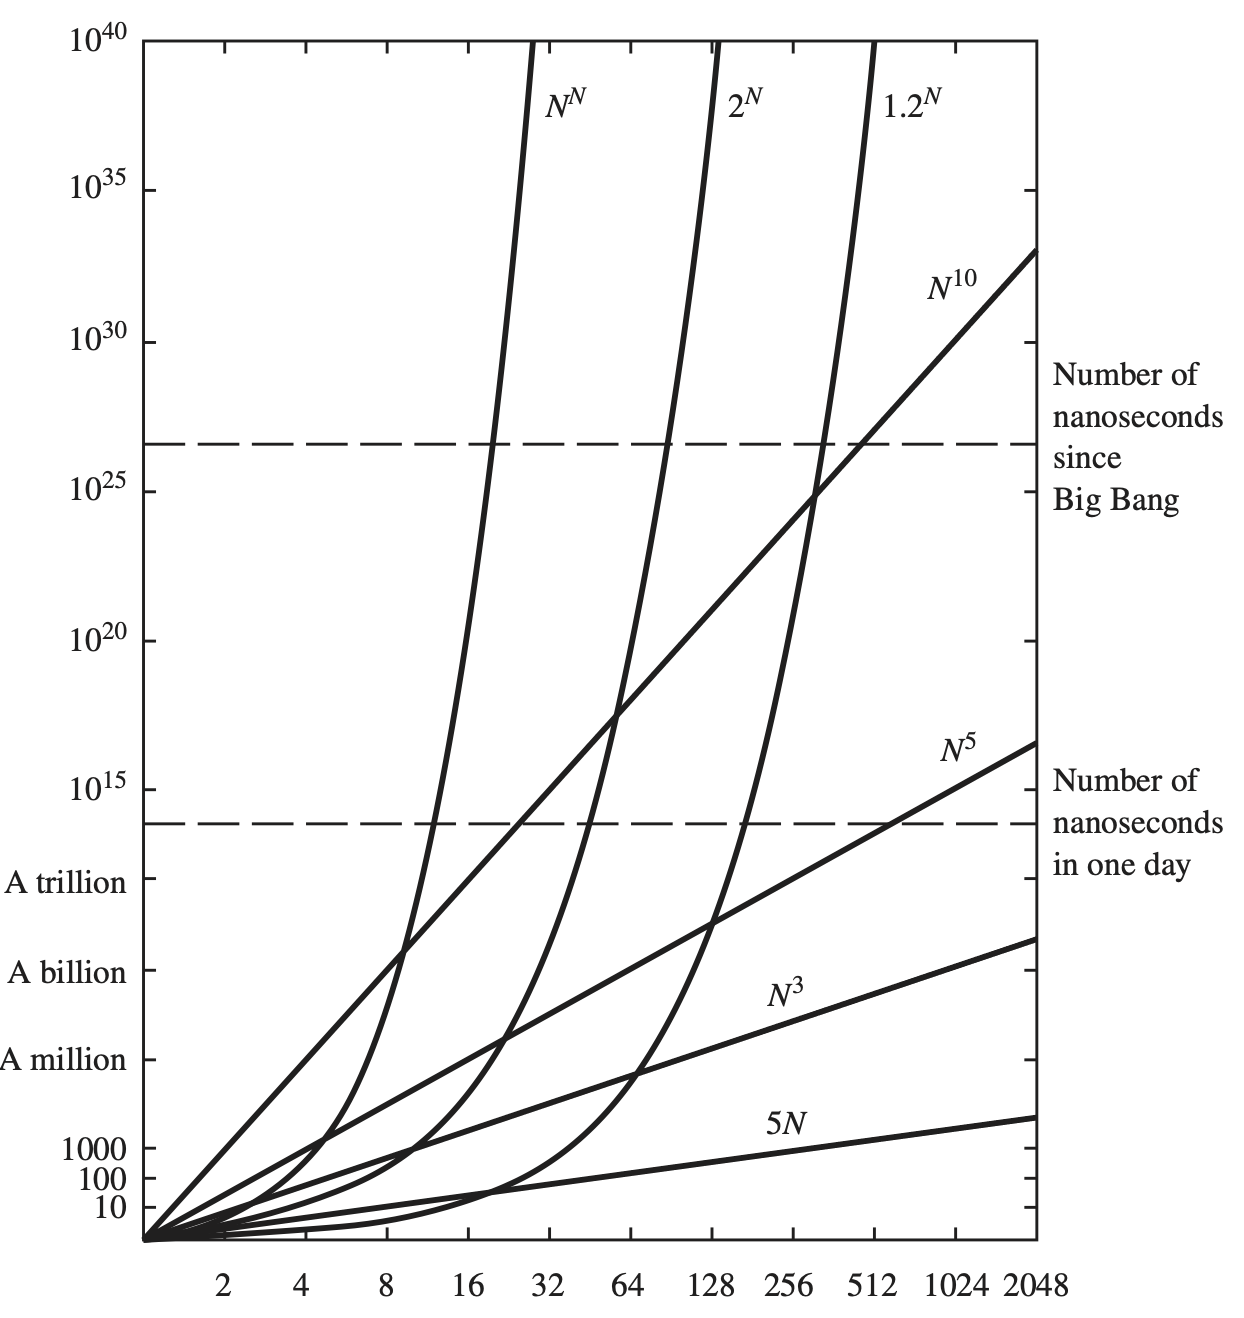
\includegraphics[width=\textwidth]{Harel2.png}
      \end{center}
    \end{column}
  \end{columns}
\end{frame}

\begin{frame}[t]{Search space complexity: the travelling salesman problem (TSP)}
  % \begin{columns}
  %   \begin{column}{0.4\textwidth}
      \begin{itemize}
        \item A salesman must visit $n$ cities
        \item Each city must be visited just once
        \item Which path should he take to minimize the total distance travelled?
      \end{itemize}
    % \end{column}
    % \begin{column}{0.4\textwidth}
      \begin{center}
        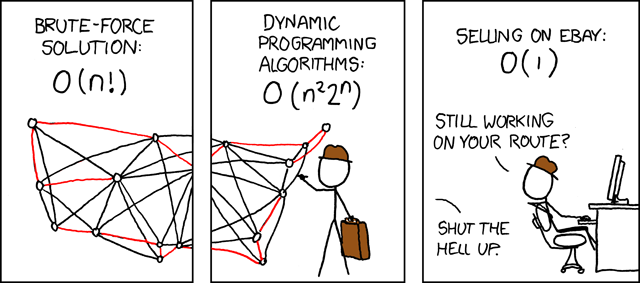
\includegraphics[width=0.7\textwidth]{XKCD_TSP.png}
      \end{center}
      \url{https://xkcd.com/399}
  %   \end{column}
  % \end{columns}
\end{frame}

\begin{frame}[t]{Search space complexity: the travelling salesman problem (TSP)}
  \begin{center}
    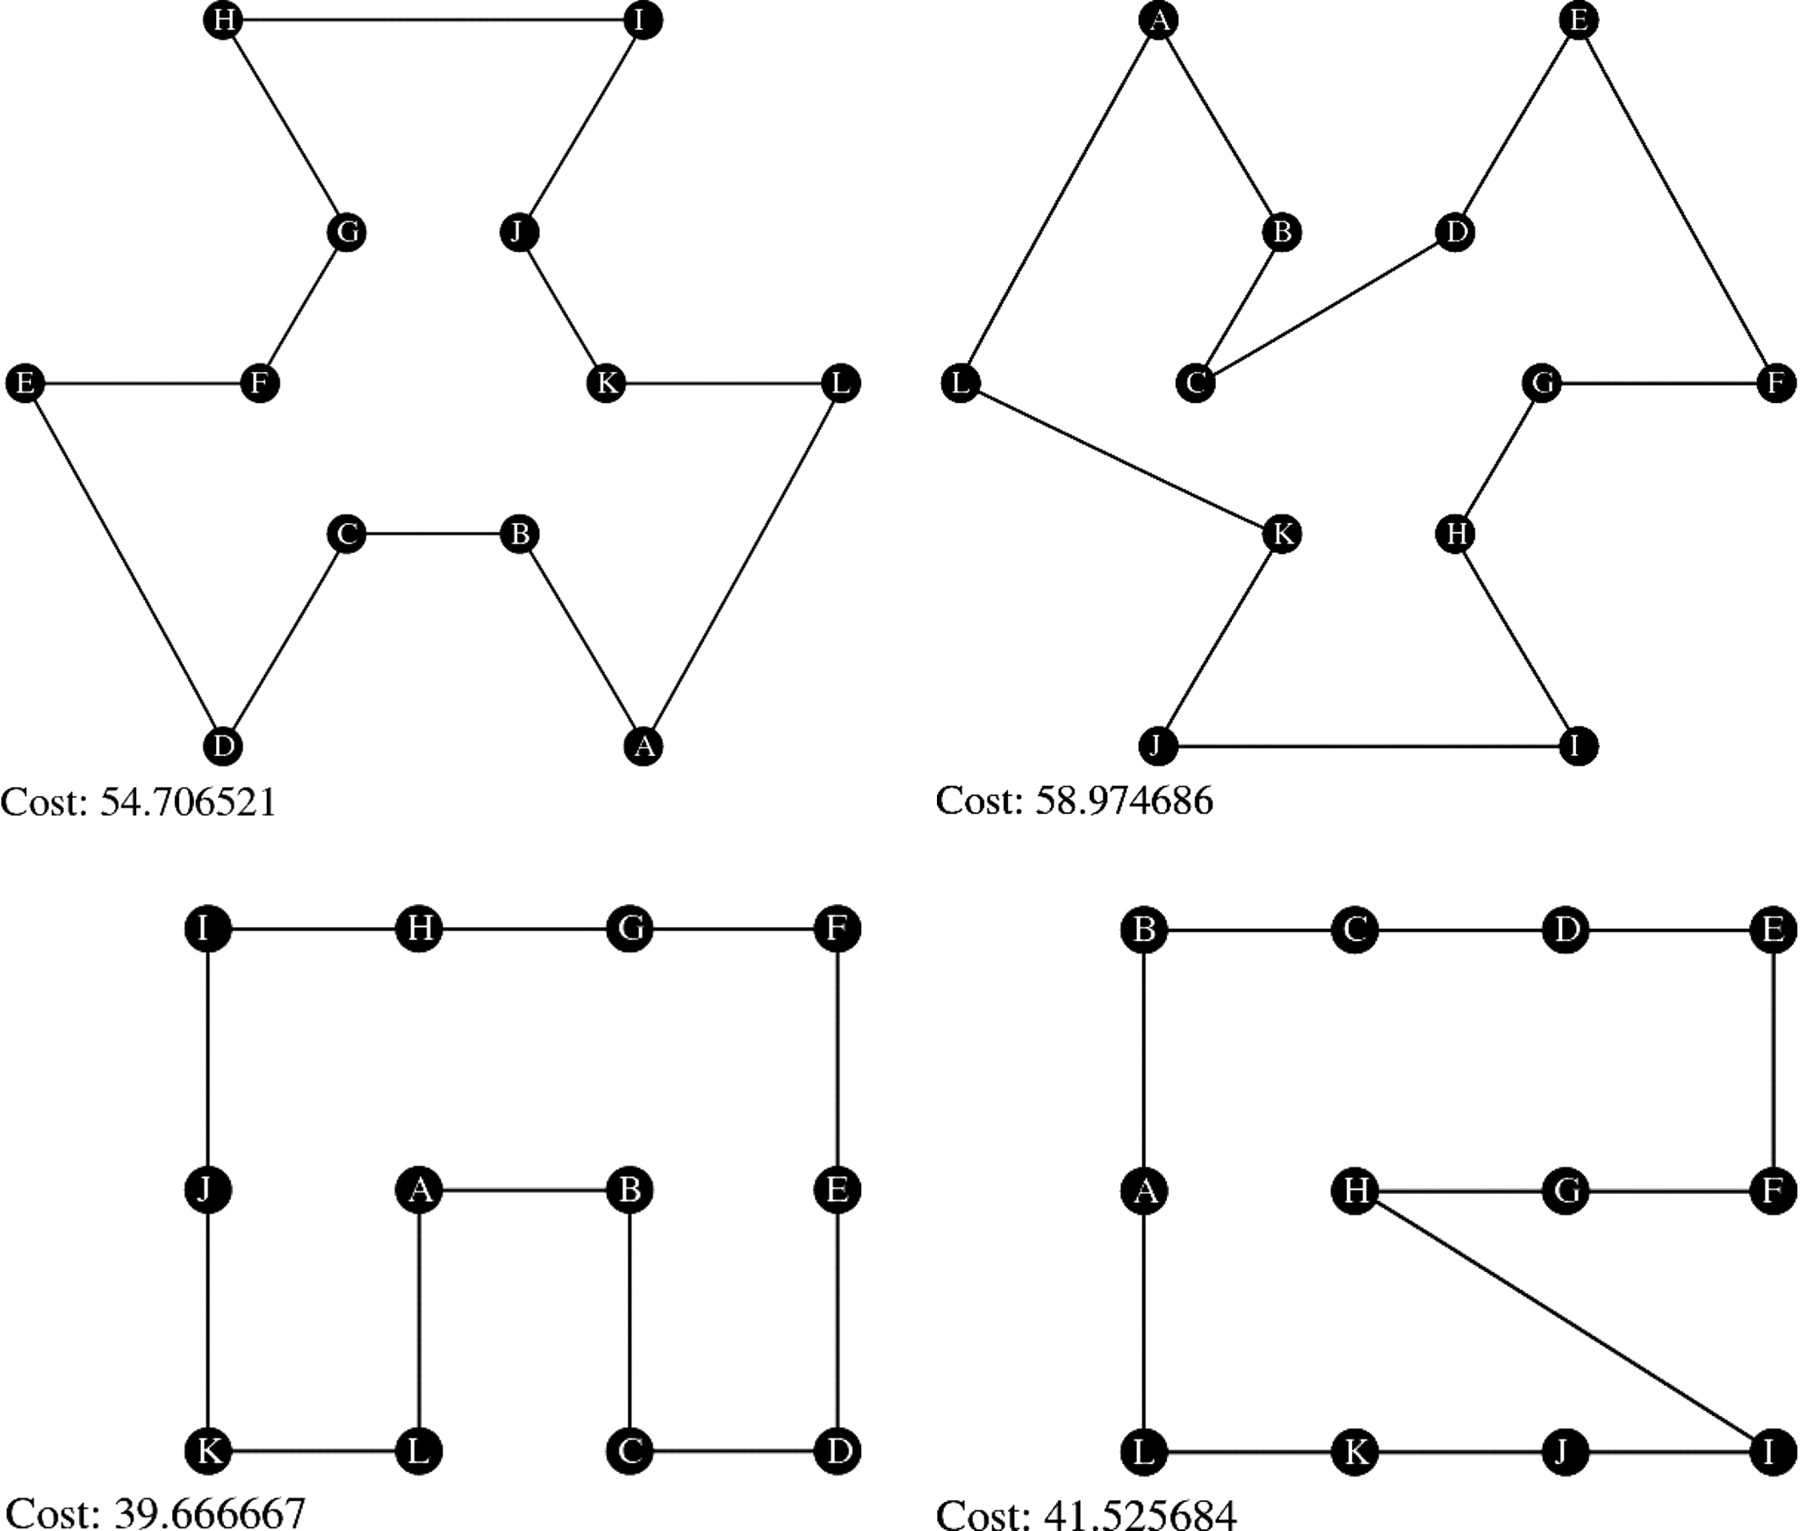
\includegraphics[width=0.5\textwidth]{TSP.jpg}
  \end{center}
  \url{https://doi.org/10.1073/pnas.0609910104}
\end{frame}

\begin{frame}{TSP practical example}
  Let us assume there are 4 cities and these are the "distances"\footnote{Note that the distance is not necessarily identical in both directions} between them:
  \begin{center}
  \begin{tabular}{c|cccc}
    $D_{ij}$ & city A & city B & city C & city D \\\hline
    city A & 0 & 5 & 10 & 20  \\
    city B & 10 & 0 & 35 & 20  \\
    city C & 20 & 10 & 0 & 5 \\
    city D & 10 & 5 & 10 & 0
  \end{tabular}
  \end{center}
  Check \href{https://github.com/JordiVillaFreixa/ORcourse/blob/main/code/TSPnaive.ipynb}{code} at GitHub 
\end{frame}

\begin{frame}{TSP practical example}
  \begin{itemize}
    \item The number of combinations is $(n-1)!$. This is the search space
    \item Asssuming a computer takes a milisecond to evaluate a solution, How long would it take for the computer to find the optimal solution in our 4 nodes problem? and how long for problems with 10, 20, 50 cities?
  \end{itemize}
\end{frame}

\begin{frame}{Optimality and Practicality}
  \begin{itemize}
    \item We have been trained in mathematics to find exact/perfect solutions. This is not always possible:
    \begin{itemize}
      \item Models are approximate representations of the real systems
      \item Accumulated round-off errors in computers
      \item Input data is usually approximated
      \item Exponential time algorithms require suboptimal solutions
    \end{itemize}
    \item "good enough" is not always lowering expectations, as the real world can be extremely complex.
  \end{itemize}
\end{frame}

\begin{frame}{Software for Operations Research}
 \begin{description}
   \item[Modeling environments] Spreadsheets (Excel, Numbers, Google), \href{https://ampl.com}{AMPL}, \href{http://www.maximalsoftware.com/mpl/}{MPL}, \href{https://www.lindo.com/index.php/products/lingo-and-optimization-modeling}{LINGO}, \href{https://www.ibm.com/docs/en/icos/12.9.0?topic=opl-optimization-programming-language}{OPL}, \href{https://www.aimms.com}{AIMMS}, \href{https://www.sas.com/es_es/software/or.html}{SAS/OR}, \href{https://support.sas.com/rnd/app/or/procedures/optmodel.html}{OPTMODEL},\href{https://www.gams.com}{GAMS}, \href{https://neos-guide.org}{NEOS}\footnote{check the \href{https://neos-guide.org/content/or}{TSP demo in NEOS/GAMS}}, ...
   \item[Solvers] \href{https://www.gurobi.com}{Gurobi},
   \href{https://www.solver.com}{Frontline Solver},
   \href{https://www.ibm.com/products/ilog-cplex-optimization-studio}{CPLEX}, ...
   \item[Software libraries] \href{https://developers.google.com/optimization}{Google OR-Tools}, \href{https://www.coin-or.org}{COIN-OR}, \href{https://www.imsl.com}{IMSL}, ...
 \end{description}
 We will be using \href{https://github.com/JordiVillaFreixa/ORcode}{Google colab} through the course when possible.
\end{frame}

%--- Next Frame ---%
%------------------------------------------------%------------------------------------------------
%------------------------------------------------%------------------------------------------------
%------------------------------------------------%------------------------------------------------
%------------------------------------------------%------------------------------------------------
%------------------------------------------------%------------------------------------------------
%------------------------------------------------%------------------------------------------------
%------------------------------------------------%------------------------------------------------
%------------------------------------------------%------------------------------------------------
%------------------------------------------------%------------------------------------------------
%------------------------------------------------%------------------------------------------------

\section{References}
\begin{frame}{References}
    \footnotesize
    \begin{thebibliography}{99}
    \setbeamertemplate{bibliography item}[text]
      \begin{columns}[t]
        \begin{column}{.45\textwidth}
            \bibitem{carter} Michael W. Carter, Camille C. Price, and Ghaith Rabadi. Operations Research, 2nd Edition. CRC Press.
            \bibitem{harel} David Harel, with Yishai Feldman. Algorithmics: the spirit of computing, 3rd Edition. Addison-Wesley.
            \bibitem{rardin} Ronald L. Rardin. Optimization in Operations Research, 2nd Edition. Pearson.
            \bibitem{hefferon} J. Hefferon. \href{http://joshua.smcvt.edu/linearalgebra}{Linear algebra (4th Ed)}.
        \end{column}
        \begin{column}{.45\textwidth}
            \bibitem{riley} K.F. Riley, M.P. Hobson, S.J. Bence. Mathematical Methods for Physics and Engineering (2nd Ed). McGraw Hill.
            \bibitem{nocedal} J. Nocedal, S. J. Wright. Numerical Optimization (2nd Ed). Springer.
            \bibitem{beers} Kenneth J. Beers. Numerical methods for chemical engineering: applications in Matlab. Cambridge University Press.
            \bibitem{barber} D. Barber. Bayesian reasoning and machine learning. Cambridge University Press.
        \end{column}
      \end{columns}
    \end{thebibliography}
\end{frame}
%----------------------------------------------------------------------------------------

\end{document}
